% +--------------------------------------------------------------------+
% | Sample Chapter 3
% +--------------------------------------------------------------------+

\cleardoublepage

% +--------------------------------------------------------------------+
% | Replace "This is Chapter 3" below with the title of your chapter.
% | LaTeX will automatically number the chapters.
% +--------------------------------------------------------------------+

\chapter{Diseño de la aplicación}
\label{makereference3}
En este capítulo pretendemos explicar cómo hemos diseñado la aplicación. Comenzaremos realizando un análisis de la competencia mediante el cual analizaremos aplicaciones que ofrezcan funcionalidades parecidas a las que nuestra 
aplicación ofrece. Continuaremos detallando una serie de escenarios reales en los que nuestra aplicación puede ser usada, a partir de estos escenarios extraeremos los requisitos funcionales. Finalmente, detallaremos las interfaces de usuario que hemos implementado.

\section{Análisis de la competencia}
\label{makereference3.1}
    Consideramos que la aplicación que hemos diseñado consta de dos funcionalidades claramente diferenciadas:
    \begin{enumerate}
    \item Realidad aumentada.
    \item Recomendación y gestión de películas.
    \end{enumerate}
    Además, pensamos que existen distintos tipos de competencia dependiendo de cada una de ellas.
     \begin{itemize}  
         \item Respecto a la funcionalidad de recomendación y gestión de películas, compite claramente con aplicaciones como IMDB\cite{imdb} o MovieBase\cite{moviebase}. 
         Estas aplicaciones proporcionan, herramientas para guardar películas y recomendar éstas a los usuarios en función de sus gustos. Estas funcionalidades son 
         muy parecidas a las que nosotros hemos decidido proporcionar a nuestros usuarios, con la diferencia que nuestra aplicación, además de las funcionalidades anteriormente 
         mencionadas, permite realizar más acciones sobre las películas como crear planes con amigos.
        \item A diferencia de la funcionalidad de recomendación y gestión en donde hay una gran variedad de aplicaciones que ofrecen servicios parecidos a los nuestros, únicamente hemos 
        encontrado una aplicación (Paramount AR+\cite{paramountar}) que ofrezca servicios parecidos a los nuestros relacionados con Realidad Aumentada. Según las especificaciones de la aplicación permite identificar pósteres y 
        mostrar información sobre la película detectada, servicio muy parecido al que nosotros hemos proporcionado. 
    \end{itemize}
    
Para intentar alejarnos de esta competencia, hemos decidido unir ambas funcionalidades en una aplicación y, además, proporcionar al usuario más funcionalidades como escanear una aplicación con Realidad Aumentada, 
 ver su información y añadirla a un plan con amigos para ver dicha película. Para funcionalidades como ésta y otras en las que unimos la realidad aumentada con la recomendación de películas y gestión de planes no hemos encontrado 
 actualmente ninguna aplicación que proporcione estos servicios.

Además, la gestión de amigos con Realidad Aumentada es una funcionalidad que, tras nuestro análisis de la competencia, solamente la posee nuestra aplicación. 
Se basa en enfocar con la cámara a un usuario de la aplicación y que mediante realidad aumentada muestre visualmente la información de los tres 
 planes activos que tiene este usuario, una vez ha sido añadido como amigo, que más podrían gustarme y cuanto se estima que me gustaría ese plan.
    
\section{Escenarios de uso}
\label{makereference3.2}
Antes de decidir como implementaríamos nuestra aplicación decidimos que sería importante establecer una serie
de escenarios en los que podría ser usada. Tras esto pudimos ponernos de acuerdo en qué funcionalidades incluiríamos y que 
éstas se ajustasen a las necesidades de los usuarios. Además, estos escenarios deberían usar la Realidad Aumentada para que 
les aporte valor, ya que, como hemos expuesto anteriormente en el \autoref{makereference2}, el grueso de nuestra aplicación se centra en esta tecnología.
Los escenarios de uso que vamos a describir a continuación son distintas situaciones del mundo real en las que los futuros usuarios de nuestra aplicación se podrían encontrar y como nuestra aplicación ayudaría a afrontar dichos escenarios. 
De esta manera, analizando las situaciones que se podrían dar en un futuro podemos extraer funcionalidades.

\paragraph{Escenario 1. Reconociendo carteles de películas.}
    Te apetece ir al cine y encuentras el cartel de una película que te interesa ver en una revista. Sacas tu móvil, abres la aplicación y 
    la escaneas. Con la realidad aumentada serás capaz de ver la valoración de la película, acceder a su tráiler en Youtube, ver la información
    referente a la película (título, director, duración, sinopsis) y guardarla como favorita.
    
\paragraph{Escenario 2. Reconociendo usuarios.}
    Has quedado con un amigo y le convences de que la aplicación es muy útil, se descarga la aplicación y le quieres añadir como amigo para realizar futuros planes. Abres la aplicación y le escaneas. Con la realidad aumentada podrás añadirle como amigo.

\paragraph{Escenario 3. Obtener recomendación.}
    Estás planeando con un amigo ver una película, sin embargo, no conseguís poneros de acuerdo en qué película ver. Abres la aplicación y escaneas a tu amigo. Mediante realidad aumentada podrás obtener la información de las películas que más os podrían gustar a los dos. 



\paragraph{Escenario 4. Quedar con amigos para ver una película.}
    Una vez que has guardado una película porque te interesa ir a verla con alguien, ya sea que quieras verla en el cine o en tu casa, sea fin de semana o no, la aplicación te facilitará quedar 
    con las personas que estén interesadas en verla, además de que la aplicación supondrá un apoyo para que los usuarios tomen sus decisiones, mostrándoles cuánta afinidad a dicha película tienen.

\paragraph{Escenario 5. Usar la aplicación sin la realidad aumentada.}
    Te apetece iniciar un plan para ir a ver una película con unos amigos, sin embargo, en ese momento no tienes la película 
    delante para poderla escanear.La aplicación te permitirá buscar 
     planes, crearlos, borrarlos y unirte a ellos, buscar películas y valorarlas y buscar usuarios y añadirlos sin hacer uso de la realidad aumentada.

\section{Requisitos funcionales}
\label{makereference3.3}
En la siguiente sección describiremos los requisitos funcionales de nuestra aplicación. Con estos requisitos pretendemos mostrar los servicios que nuestra aplicación proporcionará.
Para poder entender mejor estos servicios que proporcionaremos, hemos decidido agrupar la aplicación en cuatro grandes grupos: planes, películas, usuarios y recomendaciones.

\paragraph{\large Planes:\\}

Cuando hablamos de un plan, nos referimos a un elemento creado a partir de una película. Un plan para un usuario significa que ese usuario tiene interés en ver la película con la que se creó dicho plan.
Los planes están compuestos por una película, un usuario creador del plan, y los usuarios que se hayan unido.
\\
\textbf{Funciones:}
\begin{enumerate}
    \item Crear plan: un usuario crea un plan a partir de una película que ha guardado, con una descripción, fecha, hora y lugar determinados.
    \item Unirse a un plan: solo podrán unirse los amigos del usuario creador del plan.
    \item Salirse de un plan: una vez te has unido al plan puedes salir del mismo.
    \item Eliminar un plan: solo puede eliminar el plan la persona que lo ha creado.
    \item Información de un plan: la película que se quiere ver, los usuarios que se han unido, el usuario que lo ha creado, la fecha, el lugar, una descripción y la hora.
\end{enumerate} 
\paragraph{\large Películas guardadas:\\}

Las películas guardadas son aquellas que el usuario ha decidido guardar para ver su información más tarde o para posteriormente añadirlas a un plan.
\\
\textbf{Funciones:}
\begin{enumerate}
    \item Guardar película: cuando un usuario reconoce una película con la cámara, se le permitirá guardar la película como favorita. También podrá guardar la película si la busca desde la aplicación sin necesidad de la realidad aumentada.
    \item Información de una película: un usuario puede ver la información de una película que haya guardado. Podrá ver una pequeña sinopsis, el género, el director, su valoración y su tráiler en Youtube.
    \item Valorar una película: también se le permite a un usuario valorar una película a su gusto.
\end{enumerate} 
\paragraph{\large Usuarios:\\}
Usuario es toda aquella persona que se haya registrado en la aplicación y se haya creado un perfil.
\\
\textbf{Funciones:}
\begin{enumerate}
    \item Añadir como amigo: cuando un usuario reconoce a otro con la cámara se le permitirá añadirle como amigo. También podrá hacerlo si le busca desde la aplicación sin necesidad de la realidad aumentada.
    \item Eliminar un amigo: existe la posibilidad de eliminar a un usuario de tu lista de amigos.
    \item Información de un usuario: un usuario puede ver la información de otro usuario, como su nombre y su foto de perfil. Si son amigos podrá ver además 3 planes que le interesan a ambos.
\end{enumerate} 

\paragraph{\large Recomendaciones:\\}
Aquellas películas o planes que son afines a un cierto usuario de la aplicación según sus gustos.
\\
\textbf{Funciones:}
\begin{enumerate}
    \item Recomendar películas: al usuario de la aplicación se le recomendarán películas que se ajusten a sus gustos para que le sea más fácil tomar una decisión.
    \item Recomendar planes: cuando un usuario quiere ver una película con un amigo, se da la opción de que, enfocando al amigo mediante realidad aumentada pueda ver los planes que tiene su amigo y 
    cuanto se estima que le podrían gustar. De esta forma el usuario puede hacerse una idea de cómo de afín es a los planes de su amigo y si encaja en alguno.
\end{enumerate} 

\section{Interfaz de usuario}
\label{makereference3.4}
A continuación, describiremos las distintas interfaces de usuario que hemos realizado. En ellas hemos recogido las funcionalidades anteriormente para tratar de atender a los escenarios planteados inicialmente.
\\
Hemos dividido nuestra aplicación en 3 vistas diferentes: la interfaz de Mis planes, la de Recomendaciones y la de Mis películas. Además, poseemos una serie de interfaces de realidad aumentada que mostraremos. A continuación hablaremos
de las interfaces de usuario más relevantes que hemos diseñado:
\subsection{Interfaz principal}
\label{makereference3.4.1}
Tenemos una barra en la parte inferior para movernos por las 3 secciones de nuestra aplicación: mis planes, recomendaciones y mis películas.
Cada sección incluye un icono para apoyar a la representación.
Además, encontramos un botón con un símbolo de una cámara en todas las secciones que nos permitirá acceder a la interfaz de realidad aumentada.
\subsection{Interfaz de mis planes}
\label{makereference3.4.2}
El objetivo de esta vista es el de mostrar los planes públicos que existen, es decir, aquellos en los que estás o hayas creado, indicando con una imagen de fondo la película para la que se creó el plan, el usuario
que creó dicho plan y los usuarios que se han unido. 
Podemos observar como cada elemento representa un plan, con el fondo siendo el cartel de la película, la fecha en la que tendrá lugar el plan en la esquina superior izquierda,
justo debajo el título del plan, arriba a la derecha el número del plan (algo simple pero que nos indica
claramente lo que representa este elemento) y en la parte inferior aparecen las fotos de los usuarios que se han unido al plan.
Todo esto podemos verlo en la Figura \ref{fig:listaPlanes}.
\begin{figure}[H]
    \centering
    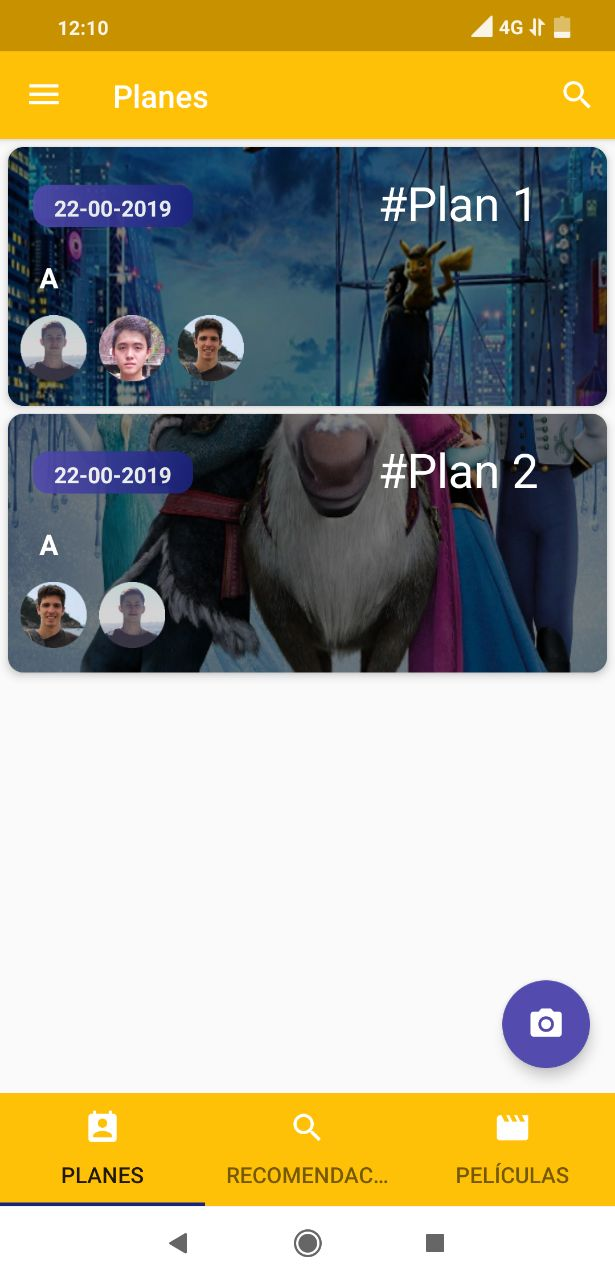
\includegraphics[height=4in]{figures/chapter-3/plan-list.jpg}
    \caption{Lista de planes}
    \label{fig:listaPlanes}
\end{figure}

\subsection{Interfaz de información de un plan}
\label{makereference3.4.3}
\begin{figure}[H]
    \centering
    \makebox[0pt][c]{%
    \begin{minipage}[b]{0.5\linewidth}
    \centering
      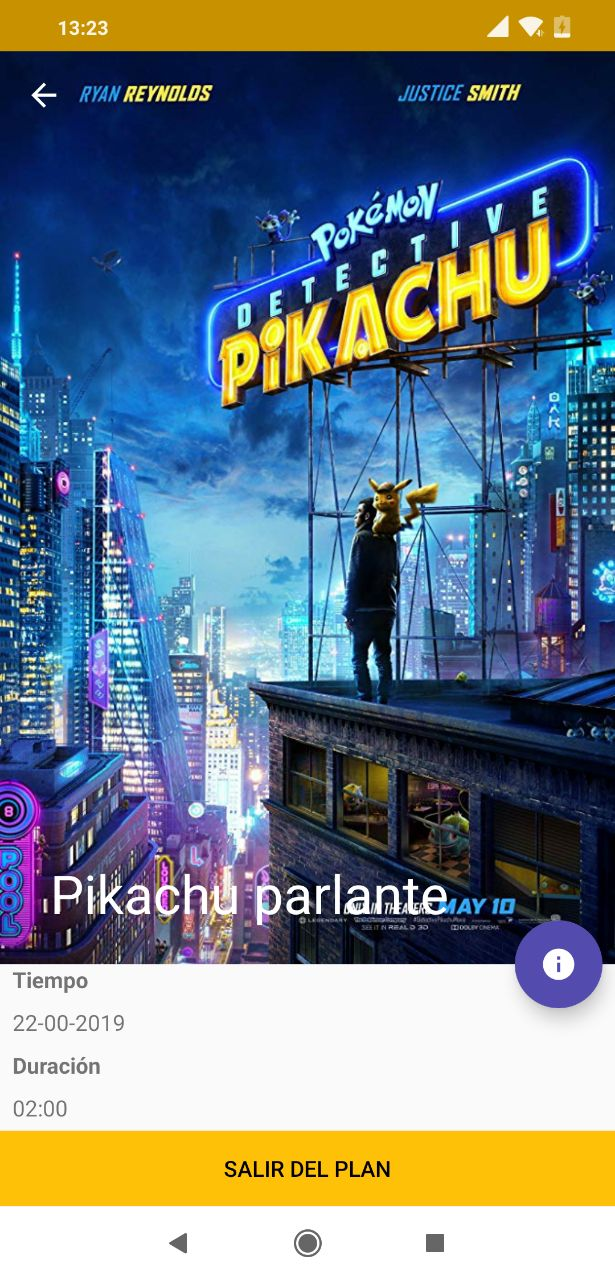
\includegraphics[height=4in]{figures/chapter-3/info-plan-extended.jpg}
      \caption{Información del plan}
    \label{fig:info_planes}
    \end{minipage}%
    \hspace{0.2cm}
    \begin{minipage}[b]{0.5\linewidth}
    \centering
     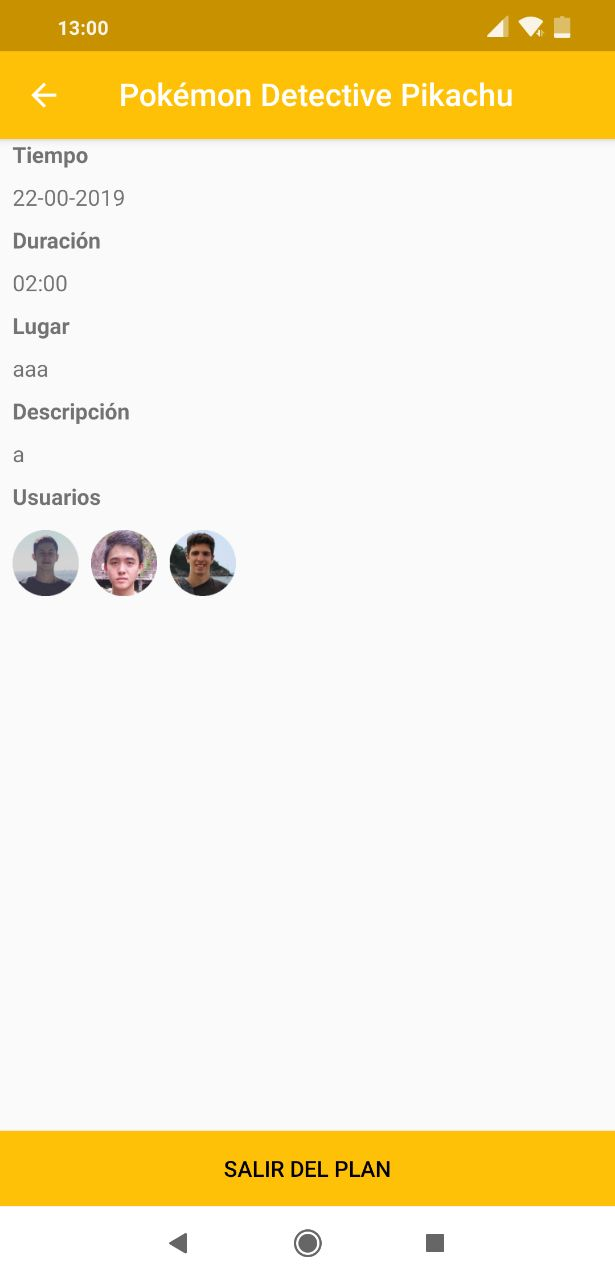
\includegraphics[height=4in]{figures/chapter-3/info-plan.jpg}
      \caption{Información del plan}
    \label{fig:info_planes_1}
    \end{minipage}%
    }%
\end{figure}
Esta interfaz aparece cuando pulsamos en un plan, (Figura \ref{fig:info_planes}). Nos aparecerá en grande la imagen de la película que se quiere ir a ver con dicho plan, junto con información
relevante de dicho plan, que podemos ver en la Figura \ref{fig:info_planes_1}:
\begin{itemize}
    \item Fecha y hora del plan.
    \item Lugar: localización que haya puesto el creador del plan para ver la película.
    \item Descripción: breves anotaciones características que haya escrito el creador sobre el plan.
    \item Usuarios unidos: imágenes de los usuarios que se han unido al plan.
\end{itemize}
\vspace{1cm}

La información de cada plan la introduce el usuario mediante un formulario muy simple cuando crea un plan con una película.
Además, nos aparece un botón en la parte inferior con el texto UNIRSE AL PLAN o SALIR DEL PLAN, según estemos o no ya dentro del plan.
También en la parte inferior derecha de la imagen de la película tenemos un botón que nos redirige a la interfaz de información de dicha película.
En la parte superior derecha nos aparecería un icono de una basura, lo que nos permitirá borrar el plan, si somos el creador.

\subsection{Interfaz Mis películas}
\label{makereference3.4.4}
Para mostrar las películas guardadas decidimos usar una cuadrícula que muestre solamente los carteles de las películas, es una interfaz simple pero muy visual. Para acceder a la información
de cada película simplemente debemos pulsar en uno de los carteles.
\begin{figure}[H]
    \centering
    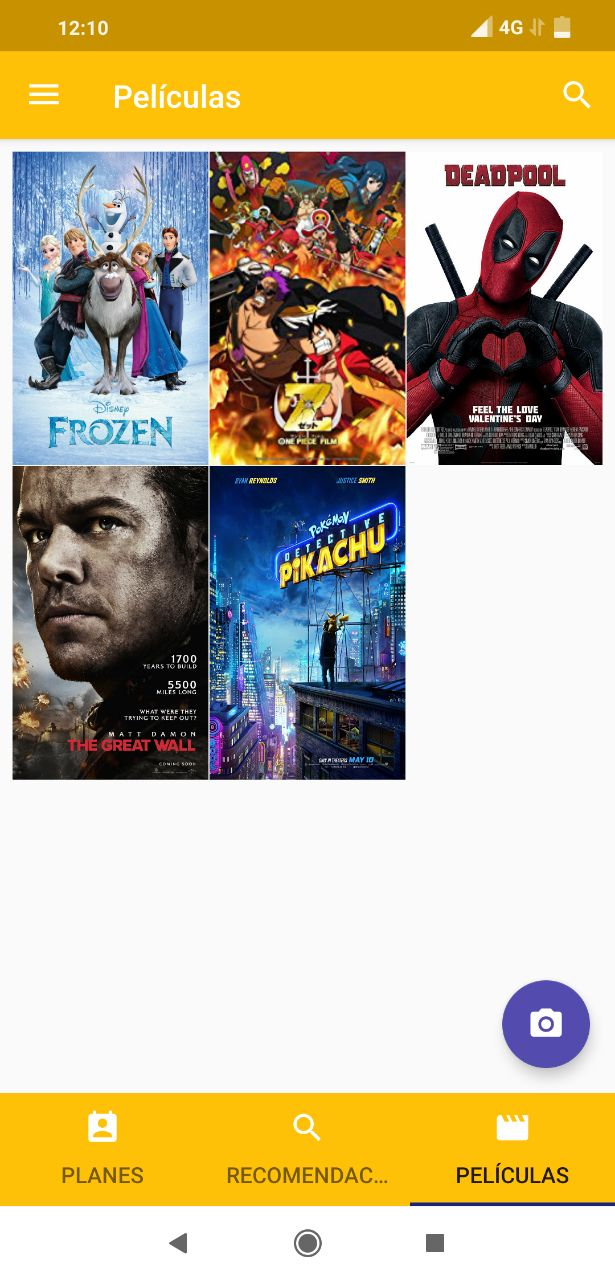
\includegraphics[height=4in]{figures/chapter-3/film-list.jpg}
    \caption{Lista de películas guardadas}
    \label{fig:lista_peliculas}
\end{figure}
En la Figura \ref{fig:lista_peliculas} podemos observar cómo es la interfaz. En este caso el usuario solo ha guardado 2 películas.
\subsection{Interfaz de información de una película}
\label{makereference3.4.5}

Tras pulsar en una de las películas que hemos guardado nos aparecerá dicha interfaz. 
Esta vista nos permite ver en primer plano el cartel de la película y la información correspondiente a la misma, como puede
ser la sinopsis de la película, el género y el nombre del director, podemos observarlo en la Figura~\ref{fig:info_pelicula_1} y la Figura~\ref{fig:info_pelicula_2}. Además, la interfaz cuenta con un indicador circular en el que 
se muestra, haciendo uso de colores, la nota de la película. Si pulsamos este, nos permite
valorar la película mediante un deslizador.
Si hacemos scroll hacia abajo, la imagen de la película se irá ocultando para ofrecernos una mejor visión de la información de la película.
En la parte inferior se nos presentan dos botones, uno para crear un plan con la película con el texto: AÑADIR AL PLAN. El otro botón con el símbolo de reproducir un vídeo, nos llevará al tráiler de la película en Youtube.
Arriba a la derecha observamos el icono de un corazón, lo que nos permitirá quitar esta película de nuestras favoritas y ya no aparecerá en la
lista de películas guardadas.

\begin{figure}[H]
    \centering
    \makebox[0pt][c]{%
    \begin{minipage}[b]{0.5\linewidth}
    \centering
      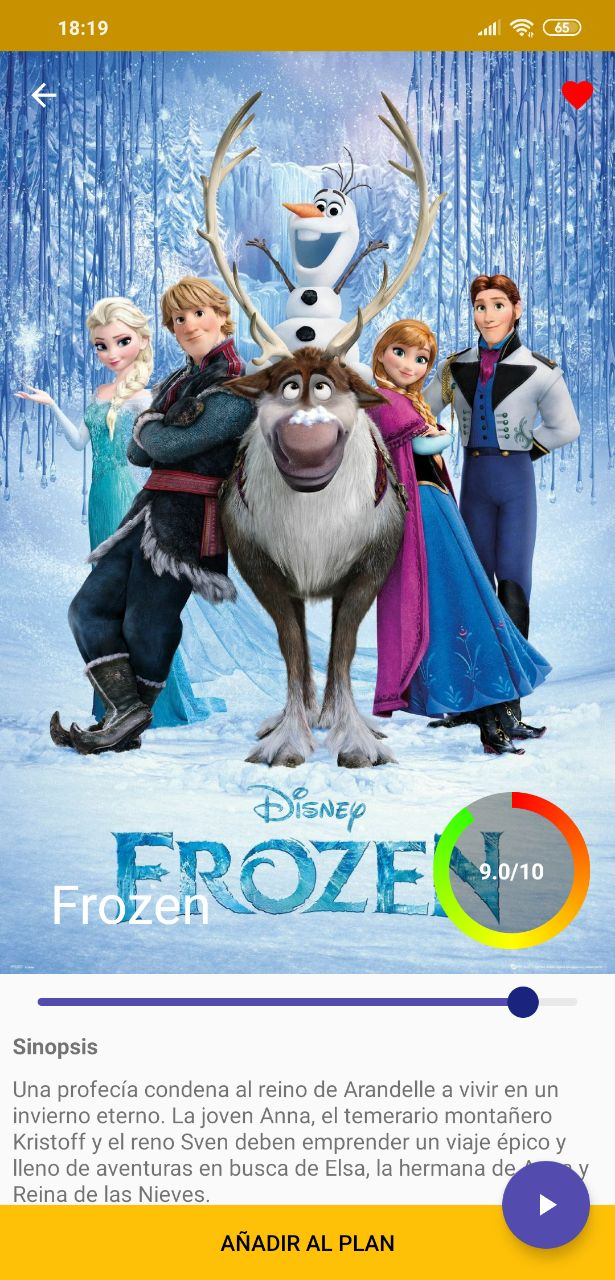
\includegraphics[height=4in]{figures/chapter-3/info-film-extended.jpg}
      \caption{Información de la película}
    \label{fig:info_pelicula_1}
    \end{minipage}%
    \hspace{0.2cm}
    \begin{minipage}[b]{0.5\linewidth}
    \centering
     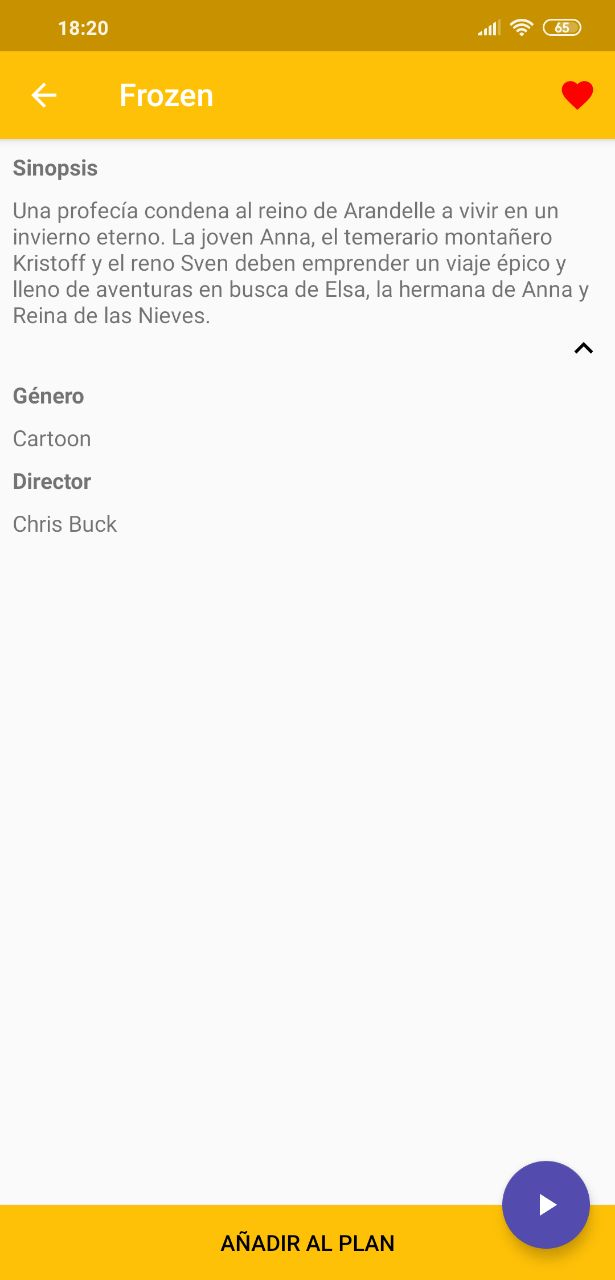
\includegraphics[height=4in]{figures/chapter-3/info-film.jpg}
      \caption{Información de la película}
    \label{fig:info_pelicula_2}
    \end{minipage}%
    }%
\end{figure}
\subsection{Interfaz Recomendaciones}
\label{makereference3.4.6}
Esta interfaz cuenta con tres secciones de recomendaciones (películas recomendadas específicamente para el usuario, películas populares y en estreno), cada una de estas secciones tiene un conjunto de carteles de 
películas que se le recomiendan al usuario.  Cada sección presenta scroll horizontal para poder
visualizar todas las películas que se le recomiendan en dicha sección, (ver en las Figuras \ref{fig:recomendaciones_1} y \ref{fig:recomendaciones_2}). La primera sección son las películas recomendadas al usuario según 
sus gustos, la segunda representa las películas más populares
y las películas que están siendo estrenadas. Al pulsar en cada una de ellas accederemos a la información de cada película (Figura \ref{fig:info_pelicula_1}) pudiendo guardarla como favorita, si no lo hemos hecho ya.
\begin{figure}[H]
    \centering
    \makebox[0pt][c]{%
    \begin{minipage}[b]{0.5\linewidth}
    \centering
      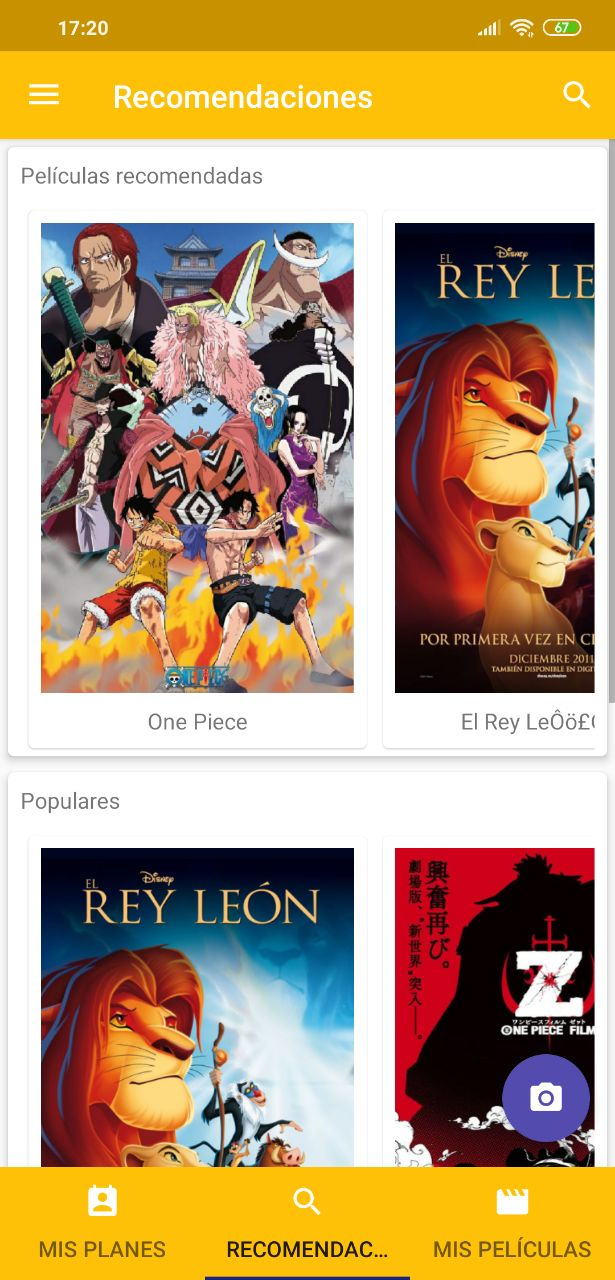
\includegraphics[height=4in]{figures/chapter-3/recommendations1.jpg}
      \caption{Recomendaciones de películas}
    \label{fig:recomendaciones_1}
    \end{minipage}%
    \hspace{0.2cm}
    \begin{minipage}[b]{0.5\linewidth}
    \centering
     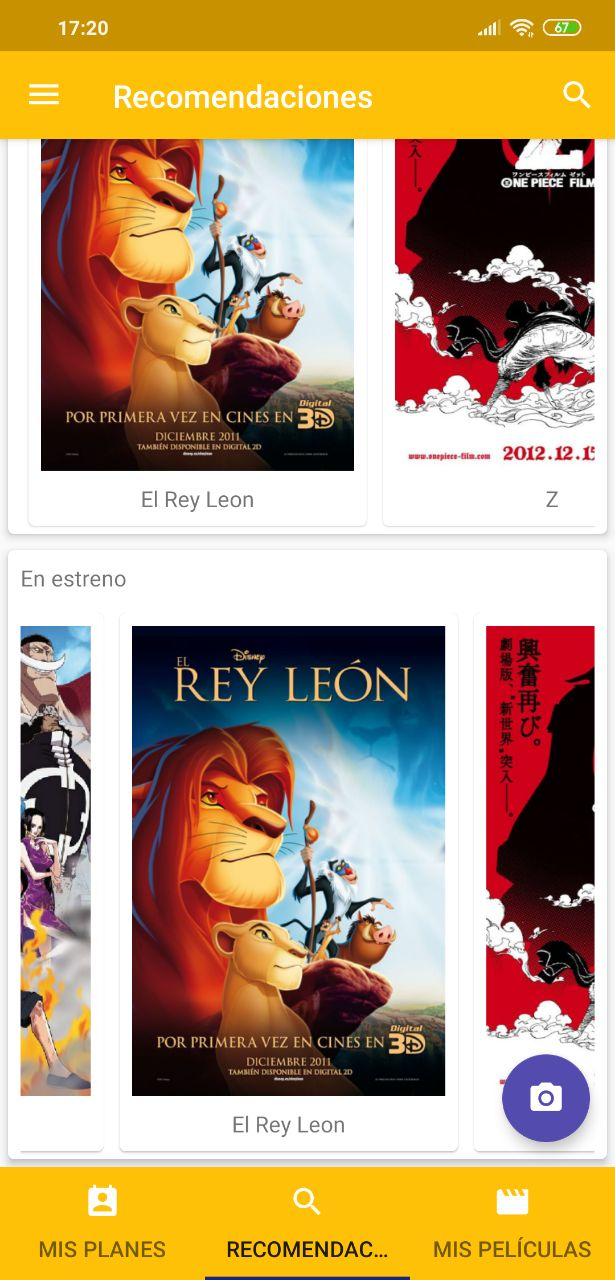
\includegraphics[height=4in]{figures/chapter-3/recommendations2.jpg}
      \caption{Recomendaciones de películas}
    \label{fig:recomendaciones_2}
    \end{minipage}%
    }%
\end{figure}

\subsection{Interfaz Usuario}
Al pulsar la foto de un amigo en cualquier lugar de la aplicación, podremos acceder a una vista de ese usuario.
En esta interfaz podremos ver la imagen del usuario, el nombre de este, los planes que tiene actualmente activos 
y el estado de nuestra relación con él. Este estado puede ser:
\begin{enumerate}
    \item Enviar petición de amistad. No hemos interactuado con este usuario y tenemos la posibilidad de enviarle 
    una petición de amistad.
    \item Esperando respuesta. Le hemos enviado en algún momento una petición de amistad y estamos esperando su respuesta.
    \item Aceptar o rechazar. El usuario en el que estamos nos ha enviado una petición de amistad y tenemos la posibilidad de 
    aceptarlo o rechazarlo.
    \item Eliminar amigo. El usuario que estamos viendo es nuestro amigo y tenemos la opción de dejar de serlo.
\end{enumerate}
\begin{figure}[H]
    \centering
    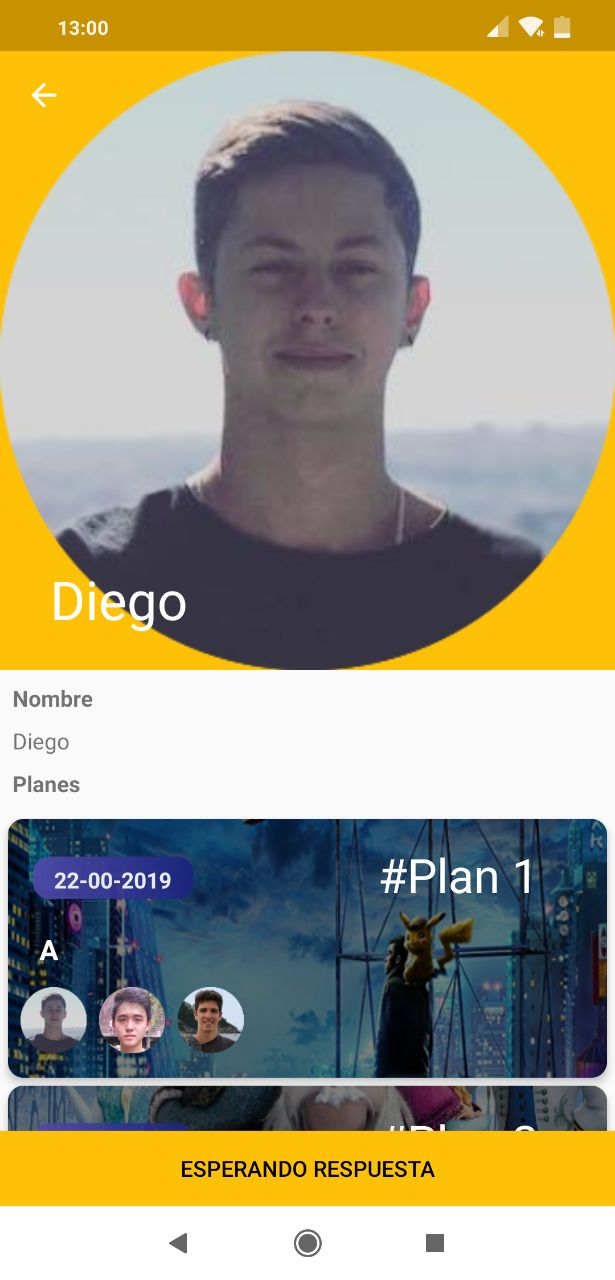
\includegraphics[height=4in]{figures/chapter-3/info-user.jpg}
    \caption{Vista de usuario}
    \label{fig:usuario}
\end{figure}
\subsection{Interfaz Lista de amigos}
Hemos decidido incorporar esta vista a nuestra aplicación ya que, es una forma muy intuitiva para que el usuario pueda ver una lista de sus amigos y usuarios a los que
ha enviado una petición de amistad.

La vista es una lista en la que se muestra la foto del amigo o usuario al que se le he enviado la petición de amistad y su nombre.
\begin{figure}[H]
    \centering
    \includegraphics[height=4in]{figures/chapter-3/listaAmigos.jpg}
    \caption{Lista de amigos}
    \label{fig:listaAmigos}
\end{figure}
\subsection{Búsquedas en las vistas}
Para facilitar al usuario el uso de la aplicación cuando haya muchos datos en esta, hemos implementado un buscador para cada una de las siguientes vistas:
\begin{enumerate}
    \item En la vista de Mis planes para permitir al usuario encontrar un plan determinado.
    \item En la vista de Recomendaciones para encontrar una película determinada.
    \item En la vista de Mis películas para, al igual que en la vista anterior, encontrar una película determinada.
\end{enumerate}
\begin{figure}[H]
    \centering
    \makebox[0pt][c]{%
    \begin{minipage}[b]{0.5\linewidth}
    \centering
      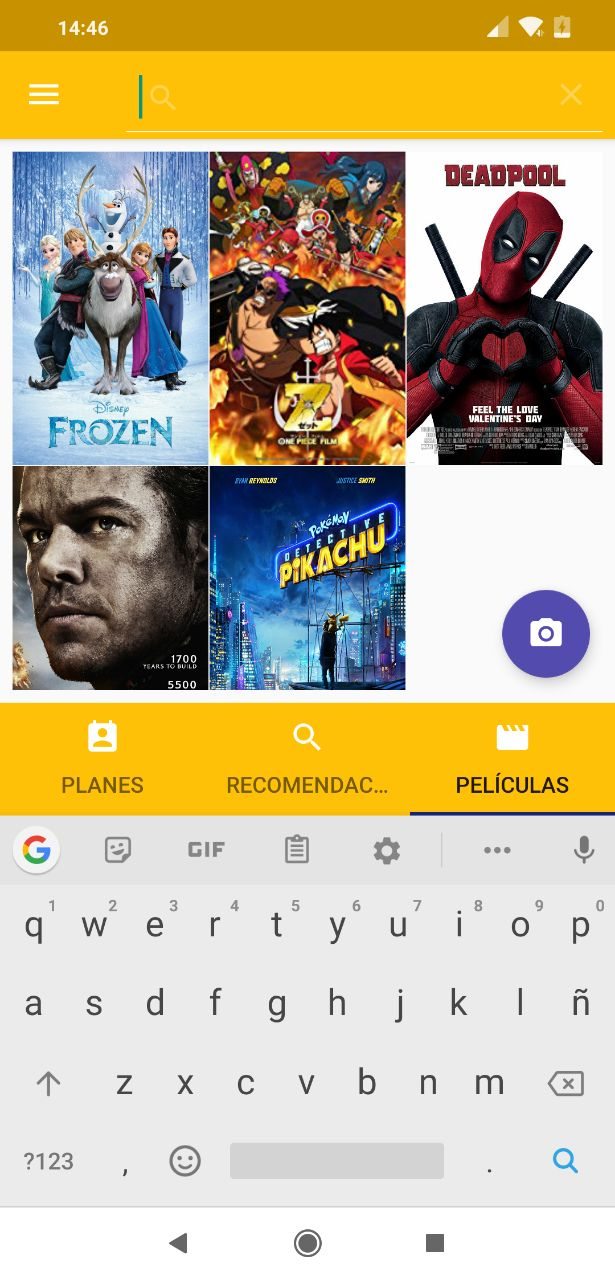
\includegraphics[height=4in]{figures/chapter-3/BuscaMisPeliculas.jpg}
      \caption{Búsqueda de Mis películas}
    \label{fig:buscaPeliculas}
    \end{minipage}%
    \hspace{0.2cm}
    \begin{minipage}[b]{0.5\linewidth}
    \centering
     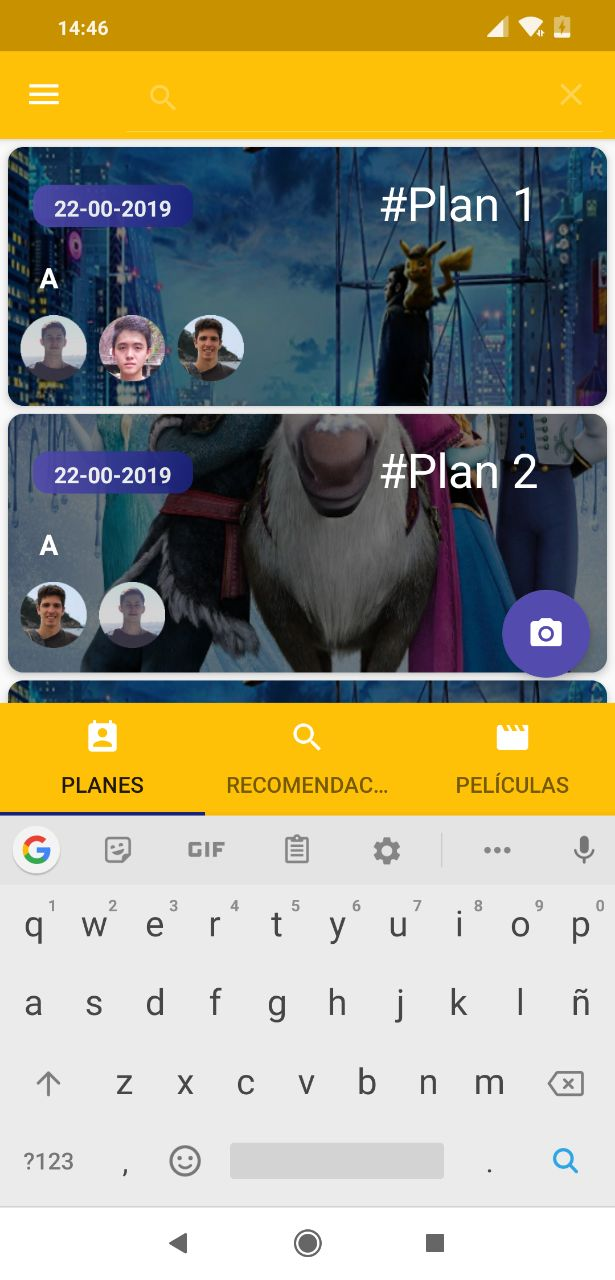
\includegraphics[height=4in]{figures/chapter-3/BuscaMisPlanes.jpg}
      \caption{Búsqueda de Mis planes}
    \label{fig:buscaPlanes}
    \end{minipage}%
    }%
\end{figure}
\subsection{Interfaz de realidad aumentada principal}
\label{makereference3.4.4}
Una interfaz muy simple en la que tenemos una línea horizontal que se mueve de arriba hacia abajo y viceversa en la pantalla como si se tratara de un escáner, para que el usuario
pueda entender que debe escanear una imagen, como podemos ver en la Figura \ref{fig:escaner}.
\begin{figure}[H]
    \centering
    
\includegraphics[height=4in]{figures/chapter-3/escaner.jpg}
    \caption{Escáner}
    \label{fig:escaner}
\end{figure}
\subsection{Interfaz de realidad aumentada tras reconocer un cartel de película}
\label{makereference3.4.5}
En esta interfaz destacamos los distintos componentes que aparecen al usar la cámara de nuestro dispositivo móvil y reconocer el cartel de una película.
Cuando reconocemos un cartel, sobre la imagen de la película nos aparecerá en la parte superior una valoración numérica de la película, la cual la hemos 
sacado de IMDB. justo en el medio de la imagen encontramos el icono típico de Youtube que, al pulsarlo, nos abrirá nuestra aplicación de Youtube para que
el usuario pueda ver el tráiler de esta película. En la esquina inferior derecha encontramos otro icono que al ser pulsado lo que hará será desplegar una serie de botones con distinta funcionalidad,
uno de ellos nos redirige a la información de la película en IMDB, que sería el icono representado por una letra i, el otro botón representado por una mano con un pulgar hacia arriba nos permitirá
guardar la película en nuestra lista de películas guardadas, para posteriormente acceder a su información, valorarla o crear un plan con ella. Todo esto lo podemos observar en la Figura \ref{fig:ra_pelicula}.

\begin{figure}[H]
    \centering
    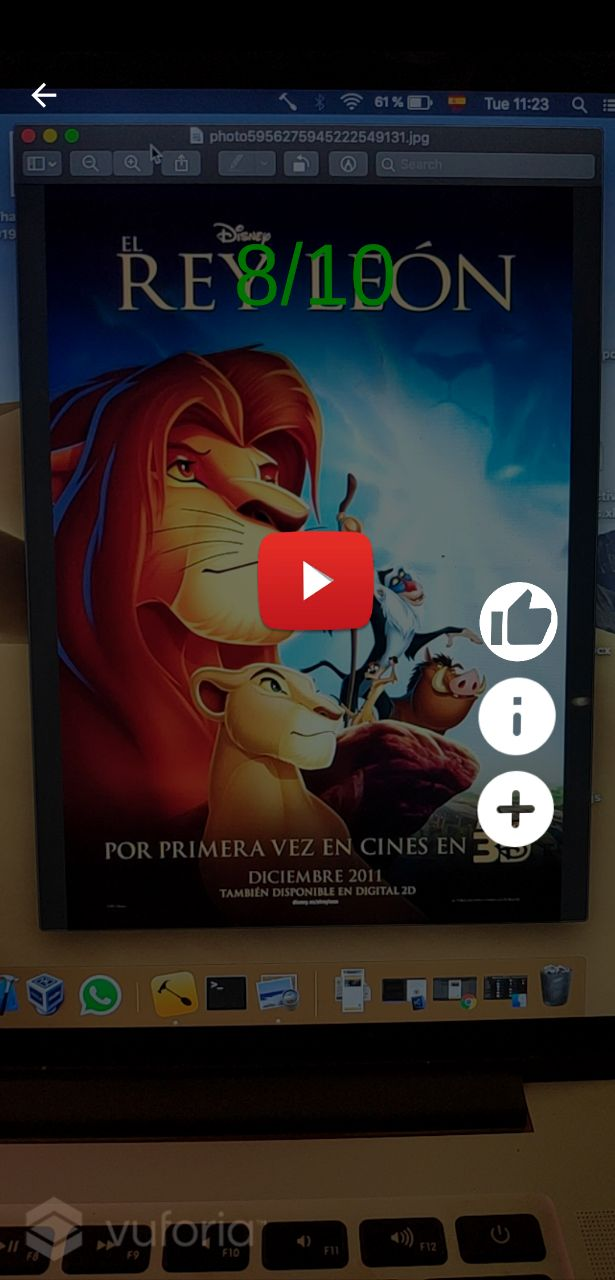
\includegraphics[height=4in]{figures/chapter-3/film-recognized.jpg}
    \caption{Realidad aumentada tras reconocer una película}
    \label{fig:ra_pelicula}
\end{figure}

\subsection{Interfaz de realidad aumentada al reconocer a un usuario que no es amigo}
\label{makereference3.4.5.1}
Se trata de una interfaz sencilla en donde a la persona que está usando la cámara, al enfocar a la imagen de otro usuario, se le proporciona el nombre del usuario al
 que está enfocando (siempre que el usuario enfocado esté registrado) junto a un botón de añadir amigo, como podemos ver en la Figura \ref{fig:ra_usuario}.
\begin{figure}[H]
    \centering
    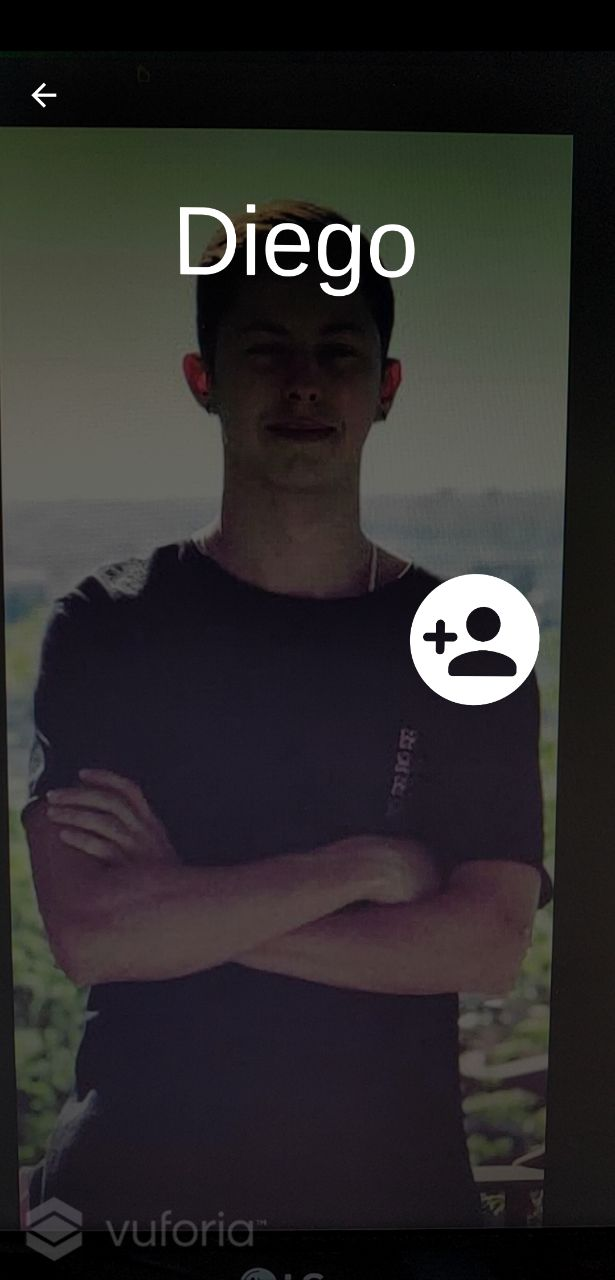
\includegraphics[height=4in]{figures/chapter-3/usernotFriendrecognized.jpg}
    \caption{Realidad aumentada tras reconocer a un usuario que no es amigo}
    \label{fig:ra_usuario}
\end{figure}
\subsection{Interfaz de realidad aumentada al reconocer a un usuario que sí es amigo}
\label{makereference3.4.5.2}
Esta interfaz aparece al enfocar con la cámara a un usuario que es amigo del que enfoca, 
es una interfaz más compleja que la anteriormente descrita.

Cuando un usuario enfoca a otro que es amigo, se proporciona la opción de incorporarse a uno de los planes del
 amigo. Para ello, se le muestra una interfaz con los tres planes que, según nuestro algoritmo de recomendación,
  más pueden interesarle de los que su amigo tiene. En caso de que haya menos de tres planes para mostrar, mostrará esos.

La interfaz proporciona la imagen de las películas de los tres planes. Además, mediante una interfaz dinámica 
podemos movernos de un plan a otro. De esta forma podemos ver qué usuarios hay en cada plan.

Al usuario al que se le están mostrando los planes de su amigo que el algoritmo le recomienda, además de los carteles de las películas, se le muestra información de los usuarios que se encuentran en cada uno de los planes.

Esta información la mostramos colocando sobre el cartel las imágenes de los usuarios que están apuntados al plan. Además, alrededor de la imagen de cada usuario se sitúa un indicador que muestra cuanto calcula el algoritmo de recomendación que le va a gustar a cada usuario el plan del que forman parte. De esta manera, el usuario que está pensando en apuntarse al plan cuenta con toda la información posible para decidir si finalmente hacerlo o no.


\begin{figure}[H]
        \centering
        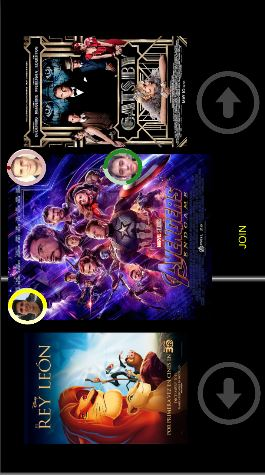
\includegraphics[width=3in, angle=270]{figures/chapter-3/CapturaRecomendador.JPG}
        \caption{Vista encargada de recomendar planes en RA al enfocar a un amigo}
        \label{fig:ra_recomendacion}
\end{figure}

Como se puede ver en la Figura \ref{fig:ra_recomendacion}, en la interfaz aparecen tres películas, esto se debe a que el recomendador ha encontrado tres planes que al usuario le pueden gustar dentro de los que el amigo al que está apuntando tiene. Únicamente se muestra la 
información relacionada con los usuarios del plan situado en el centro para no saturar la interfaz. Mediante los 
botones de izquierda y derecha el usuario puede moverse entre planes para poder ver la información necesaria 
de cada plan y elegir aquel que más le guste.


La información visual que aparece relacionada con los usuarios representa:
\begin{itemize}
    \item Arriba a la izquierda, la foto del usuario que está valorando unirse al plan, es decir, el que ha enfocado a su amigo para ver en cuál de sus planes se puede unir. Además, aparece una representación 
    gráfica de cuanto estima el algoritmo de recomendación que le puede gustar la película alrededor de su foto.
    \item Arriba a la derecha el amigo que se encuentra ya en el plan y al que se le está apuntando con la cámara. Además de la representación gráfica de cuanto estima el algoritmo de recomendación que le gusta el plan.
    \item El resto de las posiciones (hasta 6) identifican al resto de usuarios que se hayan unido a ese plan con sus fotografías y la representación gráfica de cuanto se estima que les gusta el plan del que forman parte.
\end{itemize}
Además, aparece un botón situado debajo del plan central que permite al usuario que lo pulse unirse al 
plan. Este botón mostrará una interfaz como la de la Figura \ref{fig:info_planes} y \ref{fig:info_planes_1} para que el usuario pueda ver todos 
los detalles del plan y decidir si se quiere unir.

\section{Navegación entre interfaces}
A continuación, explicaremos el diagrama mostrado en la Figura \ref{fig:navegacion}. Este diagrama muestra la manera en que se puede navegar entre las distintas interfaces
de la aplicación.
\begin{enumerate}
    \item El usuario al entrar en la aplicación accede a la vista de recomendación (Figura \ref{fig:navegacion}). Esta vista como hemos explicado anteriormente
permite navegar haciendo uso de la barra de navegación inferior, con las vistas de Planes (Figura \ref{fig:listaPlanes}) y la vista de Mis películas (Figura \ref{fig:lista_peliculas}).
    \item Presionando cualquiera de los planes mostrados en la lista de planes se accede a la vista de cada plan (Figura \ref{fig:info_planes}).
    \item Presionando alguna de las películas que aparecen en la vista de recomendaciones accedemos a la vista de cada película (Figura \ref{fig:info_pelicula_1}).
    \item Al presionar alguna de las películas de la vista de Mis películas se accede a la vista de cada película (Figura \ref{fig:info_pelicula_1}).
    \item Desde cualquiera de las vistas citadas en el punto 1 se puede acceder a la Realidad Aumentada haciendo uso del botón habilitado para ello.
    \item Al pulsar la imagen de un usuario desde cualquier vista en la aplicación, nos redirigirá a la vista de ese usuario. (Figura \ref{fig:usuario}).
    \item Una vez estamos en la Realidad Aumentada, dependiendo de a qué decidamos enfocar con la cámara accederemos a una vista u otra:
    \begin{enumerate}
        \item Al enfocar a un usuario que no es amigo se accederá a la vista en Realidad Aumentada habilitada para añadirlo como amigo. (Figura \ref{fig:ra_usuario}).
        \item Al enfocar a un usuario que sí es amigo accederemos a la interfaz en la que podremos unirnos a alguno de los planes de nuestro amigo. (Figura \ref{fig:ra_recomendacion}).
        Si finalmente decidimos unirnos a uno de sus planes, accederemos a la vista fuera de la Realidad Aumentada habilitada para ello (Figura \ref{fig:info_planes}).
        \item Al enfocar a una película, podremos ver todos los detalles de esta en Realidad Aumentada. (Figura \ref{fig:ra_pelicula}). Si decidimos ver más información de la película
        fuera de la Realidad Aumentada, al presionar el botón habilitado para ello, accederemos a la interfaz de Película (Figura \ref{fig:info_pelicula_1}).
    \end{enumerate}
\end{enumerate}

\begin{figure}[H]
    \centering
    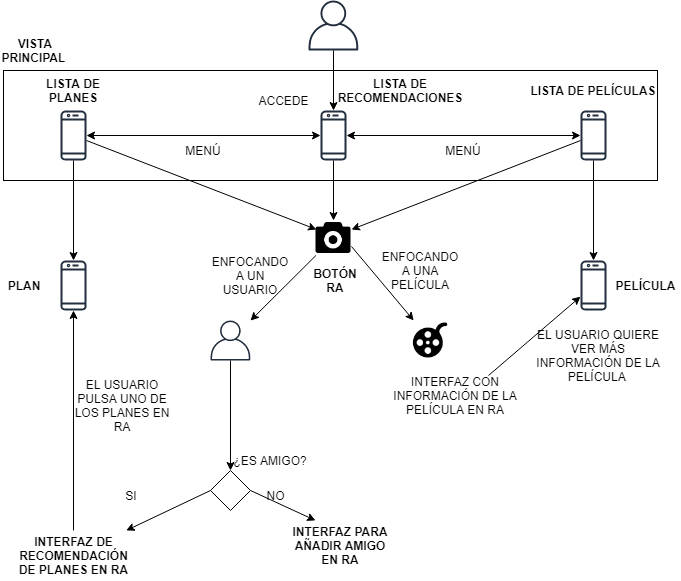
\includegraphics[width=6in]{figures/chapter-3/Navegacion.png}
    \caption{Diagrama con la navegación entre interfaces de la aplicación}
    \label{fig:navegacion}
\end{figure}

\section{Conclusiones}
En este capítulo hemos observado los distintos escenarios que hemos planteado para el uso de nuestra aplicación, a partir de ellos hemos sacado una serie de 
 requisitos funcionales que posteriormente han sido mejor especificados tras las descripciones de las interfaces de usuario que hemos diseñado, apoyándonos en imágenes 
 para mostrar visualmente a lo que nos referimos en cada subsección de las interfaces de usuario.



